\chapter{Information Extraction}

One important problem of this system is how to extract models from Job Descriptions and Resumes.
In Nature Language Processing, especially in Information Extraction, pipeline is a well adopted architecture~\cite{sarawagi2008information}. This architecture will also be used in this system to extract models of job openings and candidate's resumes. The system will process the job opening in the following steps, which is shown in Figure~\ref{fig:Pipeline}:

\begin{enumerate}
    \item HTML parser will parse the job description web pages that are obtained from web scrawler. It will get the HTML element that contains the main content of the job description.
    \item Segment module will separate the job description into paragraphs according to HTML tags at first, then separate each paragraph into sentences.
    \item The sentences will be tokenized as string array, and sent to the Classification module. Classification module will determine the category of the sentence, and mark the category of the sentence.
    \item Preprocessing module will delete unreadable characters, normalize some spelling tokens in the sentence.
    \item Annotation module will annotate the tokens with sematic and ontology labels. The sentences will be transferred to multi-layered data structure.
    \item The layered sentences will be matched with pre-defined patterns. If any pattern could be matched, the ontology information will be stored in the job model.
    \item After every sentence has be processed in the pipeline, the job model will be stored into database.
\end{enumerate}


\begin{figure}[htbp]
  \centering
  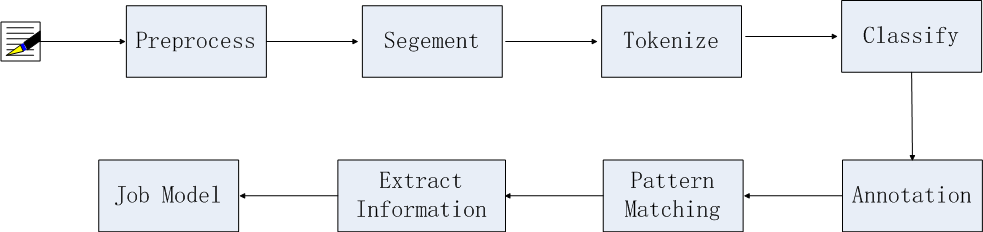
\includegraphics[scale=0.4]{images/pipeline.png}
  \caption{Job Description Process Pipeline}
  \label{fig:Pipeline}
\end{figure}
